\section{Part 2}\label{sec:02_part2}

\subsection{Introduction}\label{subsec:02_part2_intro}
% Short intro
In addition to the \textit{TinyHttpd}, dynamic pages have been introduced in the lecture. In detail, the Common Gateway Interface (CGI) has been introduced, which is able to spawn processes on the server, and send the result as a HTTP response.
% Problem statement
The task of this part of the assignment, is to create a script, that performs the \textit{StringReverser} application, as introduced in \Sec{subsubsec:01_part1_design_stringreverser}, and send the result via HTTP. This task is almost equally to the first task (introduced in \Sec{subsec:01_part1_intro}), but rather than extending an existing Java project, a script has to be created which will be launched within the \texttt{cgi-bin} folder of the Apache Web Server.
% Apache
For this task, the Apache Web Server is an requirement and the version XAMPP 7.4.23 for Mac is being used. 

\subsection{Conceptual Design}\label{subsec:02_part2_design}
% What does the script
Given the previously introduced problem statement in \Sec{subsec:02_part2_intro}, a script will be implemented using bash. Therefore, the environment variables can be used, to read details about the HTTP request.
% Procedure
Overall, the script has the same requirements, as the modification of the first task. However, the client can send a request via the url \path{http://localhost:80/cgi-bin/run_reverse_process.sh?param=ROMA}. Therefore, the use case is limited to the reverse process.

\subsection{Implementation}\label{subsec:02_part2_impl}
% Explain implementation
The implementation of the script is available at \Lst{lst:02_part2_impl_script}.
% Steps
The script is implemented in accordance to the following steps:
\begin{enumerate}
\item Check if the request was send via GET
\item Verify if a query is given
\item Validate the given query
\item If the given query is valid, perform the \textit{StringReverser} Java process and send the process output to the client via HTTP
\end{enumerate}
% chmod
It is important to mention, that the priviliges of the script has to be changed with \texttt{\$ chmod +x SCRIPT\_PATH} to make it executable.


% First
A simple if statement is used to check if the request was send via the GET method, otherwise an error message is sent. The request method is available via the environment variable \texttt{\$REQUEST\_METHOD}.


% Query
In the next step, the query has to be validated, which is saved in the environment variable \texttt{\$QUERY\_STRING}. If \texttt{\$QUERY\_STRING} is either not set or empty, an error message is sent by the script, which is illustrated in \Fig{fig:02_part2_impl_failure1}.

% failure 1 response
\begin{figure}[h]
\centering
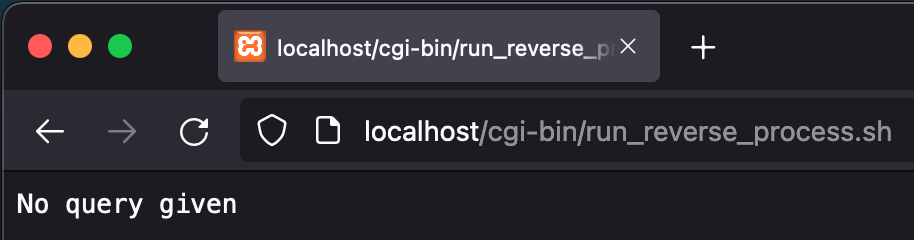
\includegraphics[scale=0.6]{images/part2Failure1}
\caption{The error message if no query is provided}
\label{fig:02_part2_impl_failure1}
\end{figure}

% Get the string
After the query string has been validated accordingly, the value of the first parameter has to be extracted. This is done by splitting the query string into its single parts. Next, the script checks if the value of the first parameter is valid. If not, an error message is sent to client, as illustrated in \Fig{fig:02_part2_impl_failure2}.

% failure 2 response
\begin{figure}[h]
\centering
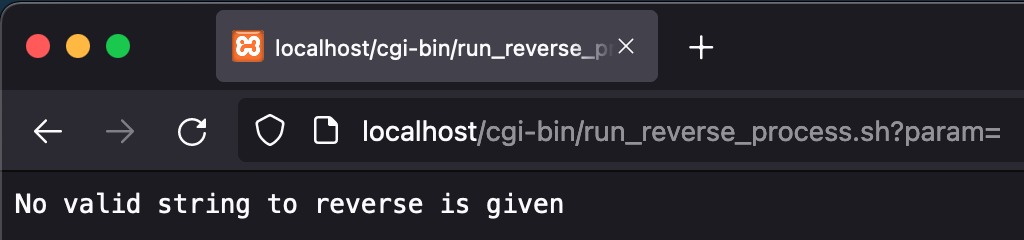
\includegraphics[scale=0.6]{images/part2Failure2}
\caption{The error message if the query is invalid}
\label{fig:02_part2_impl_failure2}
\end{figure}

% Now execute
The last step, is to execute the \textit{StringReverser} application by executing it via the command \texttt{java -jar ARTIFACT\_PATH STRING\_TO\_REVERSE}. Therefore, the generated \texttt{.jar} artifact is placed in the \texttt{cgi-bin/} directory of the Apache installation. After the process has been executed successfully, the output is send to the client as a HTTP response with the MIME type \texttt{text/plain}. This is shown in \Fig{fig:02_part2_impl_success}.

% successful response
\begin{figure}[h]
\centering
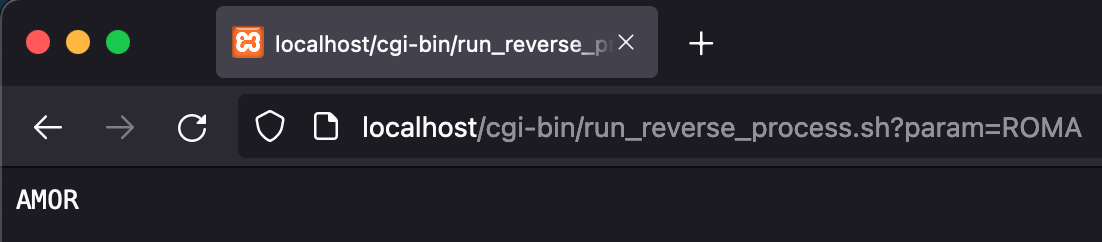
\includegraphics[scale=0.6]{images/part2Success}
\caption{A successful process request using the cgi-bin script}
\label{fig:02_part2_impl_success}
\end{figure}

\subsection{Problems}\label{subsec:02_part2_concl}
% A problem
A problem during the implementation was, that the Apache Web Server had no rights to execute Java processes. The solution to this problem, is to set a user with rights to execute a Java process, instead of the \textit{deamon} user. This can be set in the \path{httpd.conf} file of the Apache installation directory.